% Full instructions available at:
% https://github.com/elauksap/focus-beamertheme

\documentclass[9pt]{beamer}
\usetheme{focus}

%%%%%%%%%%%%%%%%%%%%%%%%%%%%%%%%%%%%%%%%%%%%%%%%%%%%%%%%%%%%%%%%%%%%%
% Typography, change document font
\usepackage[tt=false, type1=true]{libertine}
\usepackage[varqu]{zi4}
\usepackage[libertine]{newtxmath}
\usepackage[T1]{fontenc}

\usepackage[protrusion=true,expansion=true]{microtype}

% Disable paragraph indentation, and increase gap
\usepackage{parskip}

%Matrix
\usepackage{tabstackengine}
\setstackEOL{;}% row separator
\setstackTAB{,}% column separator
\setstacktabbedgap{1ex}% inter-column gap 
\setstackgap{L}{1.0\normalbaselineskip}% inter-row baselineskip
\let\mat\bracketMatrixstack

\newcommand{\pth}{Figure/}
\newcommand{\ve}[1]{\mathbf{#1}}

% Copyright (C) 2018-2019 Pasquale Claudio Africa and the LaTeX community.
% A full list of contributors can be found at
%
%     https://github.com/elauksap/focus-beamertheme
% 
% This file is part of beamerthemefocus.
% 
% beamerthemefocus is free software: you can redistribute it and/or modify
% it under the terms of the GNU General Public License as published by
% the Free Software Foundation, either version 3 of the License, or
% (at your option) any later version.
% 
% beamerthemefocus is distributed in the hope that it will be useful,
% but WITHOUT ANY WARRANTY; without even the implied warranty of
% MERCHANTABILITY or FITNESS FOR A PARTICULAR PURPOSE. See the
% GNU General Public License for more details.
% 
% You should have received a copy of the GNU General Public License
% along with beamerthemefocus. If not, see <http://www.gnu.org/licenses/>.

\mode<presentation>


% DEFINE COLORS. ---------------------------------------------------------------
\definecolor{main}{RGB}{134, 161, 174}
\definecolor{main2}{RGB}{104, 131, 144}
\definecolor{textc}{RGB}{20, 20, 20}
\definecolor{background}{RGB}{255, 255, 255}

\definecolor{alert}{RGB}{180, 0, 0}
\definecolor{example}{RGB}{0, 110, 0}


% SET COLORS. ------------------------------------------------------------------
\setbeamercolor{normal text}{fg=textc, bg=background}
\setbeamercolor{alerted text}{fg=textc}
\setbeamercolor{example text}{fg=textc}

\setbeamercolor{titlelike}{fg=background, bg=main}
\setbeamercolor{frametitle}{parent={titlelike}}

\setbeamercolor{footline}{fg=background, bg=main2}

\setbeamercolor{block title}{bg=main!80!background, fg=background}
\setbeamercolor{block body}{bg=main!10!background, fg=textc}

\setbeamercolor{block title alerted}{bg=alert, fg=background}
\setbeamercolor{block body alerted}{bg=alert!10!background, fg=textc}

\setbeamercolor{block title example}{bg=example, fg=background}
\setbeamercolor{block body example}{bg=example!10!background, fg=textc}

\setbeamercolor{itemize item}{fg=textc}
\setbeamercolor{itemize subitem}{fg=textc}

\setbeamercolor{enumerate item}{fg=textc!70!black}
\setbeamercolor{enumerate subitem}{fg=textc!70!black}

\setbeamercolor{description item}{fg=textc!70!black}
\setbeamercolor{description subitem}{fg=textc!70!black}

\setbeamercolor{caption name}{fg=textc}

\setbeamercolor{section in toc}{fg=textc}
\setbeamercolor{subsection in toc}{fg=textc}
\setbeamercolor{section number projected}{bg=textc}
\setbeamercolor{subsection number projected}{bg=textc}

\setbeamercolor{bibliography item}{fg=main}
\setbeamercolor{bibliography entry author}{fg=main!70!black}
\setbeamercolor{bibliography entry title}{fg=main}
\setbeamercolor{bibliography entry location}{fg=main}
\setbeamercolor{bibliography entry note}{fg=main}

\mode<all>


\begin{document}
	\tableofcontents


\section{Plates : \today}

	\begin{frame}
		\begin{itemize}
			\item Plate has large dimension compared to thickness. No need to use 3D, with study the deformations and stresses in plates, smal rotations and large displacement (w/h>1)
			\item Extension of Euler berunoulli is called Kirchoff plate. Extension of timoshenko beam is the first order or mindlin shear deformation plate theory.
			\item $\ve{X}$ is used for the material coordinates and $\ve{x}$ is used for the spatial coordinates. No distinction is made between the material and spatial coordinates. 	
		\end{itemize}
	\end{frame}


	\begin{frame}{Classical plate theory}
		The disp satisfy the kirchoff rules which are an extension of the euler bernoulli hypothesis which are
		\begin{itemize}
			\item Straight lines perpendicular to the mid surface remain straight
			\item Transverse normals do not have elongation
			\item Cross sections remain perpendiuclar under rotation
		\end{itemize}
	\end{frame}


	\begin{frame}{Dislacement and strain fields}
		\begin{itemize}
			\item We have the domain of the plate as $\Omega_o \times (-h/2,h/2)$. The boundary of the top surface $z = h/2$ and bottom surface $z = -h/2$ with boundary $\Gamma$ which is a curved surface with outward normal $\ve{n} = n_xe_1 + n_ye_2$
			\begin{figure}
				\centering
				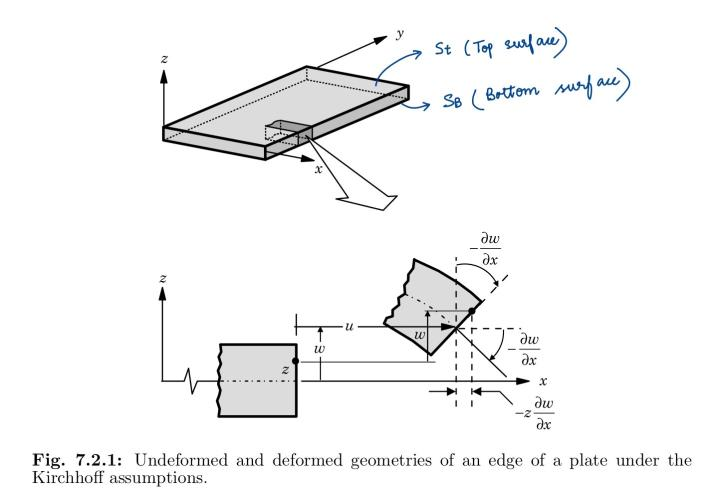
\includegraphics[width=0.8 \linewidth]{Figure/fig30} 		
			\end{figure}
		\end{itemize}
	\end{frame}


	\begin{frame}
		\begin{itemize}
			\item The kirchoff hypotehesis implies the following displacement field 
			\begin{equation}
			\begin{aligned}
				u_1(x,y,z,t) = u(x,y,t) - z\frac{\partial w}{\partial x} \\
				u_2(x,y,z,t) = v(x,y,t) - z\frac{\partial w}{\partial y} \\
				u_3(x,y,z,t) = w(x,y,t) 
			\end{aligned}
			\end{equation}
			\item Where $u,v,w$ denote the material point in the undeformed of the nerutral axis wherees $u_1,u_2,u_3$ denote any aribitary point location
			\item The componenets of the Green-Lagrange strain tensor $\ve{E}$ in terms of components of the total displacement vector $u = x(x,t) - X$ (x and X here are the same) is
			\begin{equation}
				\tiny
				\begin{aligned}
					E_{11} = \frac{\partial u_1}{\partial X_1} + \frac{1}{2}\left[ \left(\frac{\partial u_1}{\partial X_1} \right)^2 +
					\left(\frac{\partial u_2}{\partial X_1} \right)^2 + 
					\left(\frac{\partial u_3}{\partial X_1} \right)^2 \right] \\ 
					E_{22} = \frac{\partial u_2}{\partial X_2} + \frac{1}{2}\left[ \left(\frac{\partial u_1}{\partial X_2} \right)^2 +
					\left(\frac{\partial u_2}{\partial X_2} \right)^2 + 
					\left(\frac{\partial u_3}{\partial X_2} \right)^2 \right]\\
					E_{33} = \frac{\partial u_3}{\partial X_3} + \frac{1}{2}\left[ \left(\frac{\partial u_1}{\partial X_3} \right)^2 +
					\left(\frac{\partial u_2}{\partial X_3} \right)^2 + 
					\left(\frac{\partial u_3}{\partial X_3} \right)^2 \right]\\
					E_{12} = \frac{1}{2}\left[ \frac{\partial u_1}{\partial X_2} + \frac{\partial u_2}{\partial X_1} + 
					\frac{\partial u_1}{\partial X_1}\frac{\partial u_1}{\partial X_2} +
					\frac{\partial u_2}{\partial X_1}\frac{\partial u_2}{\partial X_2} +
					\frac{\partial u_3}{\partial X_1}\frac{\partial u_3}{\partial X_2} +
					\right]	\\
					E_{13} = \frac{1}{2}\left[ \frac{\partial u_1}{\partial X_3} + \frac{\partial u_3}{\partial X_1} + 
					\frac{\partial u_1}{\partial X_1}\frac{\partial u_1}{\partial X_3} +
					\frac{\partial u_2}{\partial X_1}\frac{\partial u_2}{\partial X_3} +
					\frac{\partial u_3}{\partial X_1}\frac{\partial u_3}{\partial X_3} +
					\right]	\\
					E_{23} = \frac{1}{2}\left[ \frac{\partial u_2}{\partial X_3} + \frac{\partial u_3}{\partial X_2} + 
					\frac{\partial u_1}{\partial X_2}\frac{\partial u_1}{\partial X_3} +
					\frac{\partial u_2}{\partial X_2}\frac{\partial u_2}{\partial X_3} +
					\frac{\partial u_3}{\partial X_2}\frac{\partial u_3}{\partial X_3} +
					\right]	
				\end{aligned}
			\end{equation}
		\end{itemize}
	\end{frame}


	\begin{frame}
		\begin{itemize}
			\item If the components of the displacement gradient are very small = O($\epsilon$), then the terms having O($\epsilon^2$) can be omitted in the strains. However if the rotations of the transverse normals are moderate (10 -15 degrees), then the following strains are small but not negligible
			\begin{equation}
			\left(\frac{\partial u_3}{\partial X_1} \right)^2 \qquad
			\left(\frac{\partial u_3}{\partial X_2} \right)^2 \qquad
			\frac{\partial u_3}{\partial X_1}\frac{\partial u_3}{\partial X_2}  
			\end{equation}
			\item  Thus the strains take the following (Remember that $E = \varepsilon$ where we say its small strain but moderate rotations)
			\begin{equation}
			\tiny
			\begin{aligned}
			E_{11} = \varepsilon_{11}= \frac{\partial u_1}{\partial x} + \frac{1}{2}\left[ \left(\frac{\partial u_3}{\partial x} \right)^2 \right] \qquad
			E_{22} = \frac{\partial u_2}{\partial y} + \frac{1}{2}\left[ 
			\left(\frac{\partial u_3}{\partial y} \right)^2 \right]\\
			E_{33} = \frac{\partial u_3}{\partial z} \qquad
			E_{12} = \frac{1}{2}\left[ \frac{\partial u_1}{\partial y} + \frac{\partial u_2}{\partial x} + 
			\frac{\partial u_3}{\partial x}\frac{\partial u_3}{\partial y} 
			\right]	\\
			E_{13} = \frac{1}{2}\left[ \frac{\partial u_1}{\partial z} + \frac{\partial u_3}{\partial x} 
			\right]	\qquad
			E_{23} = \frac{1}{2}\left[ \frac{\partial u_2}{\partial z} + \frac{\partial u_3}{\partial y}
			\right]	
			\end{aligned}
			\end{equation}
		\end{itemize}
	\end{frame}


	\begin{frame}
		\begin{itemize}
			\item  For this displacement field, we have $\varepsilon_{z} = \frac{\partial u_3}{\partial z} = \frac{\partial w}{\partial z} = 0$ and taking the displacement fields. The strains then reduce to
			\begin{equation}
				\begin{aligned}
				\varepsilon_{xx}= \frac{\partial u}{\partial x} + \frac{1}{2}\left[ \left(\frac{\partial w}{\partial x} \right)^2 - z \frac{\partial^2 w}{\partial x^2}\right] \qquad
				\varepsilon_{yy} = \frac{\partial v}{\partial y} + \frac{1}{2}\left[ 
				\left(\frac{\partial w}{\partial y} \right)^2 - z\frac{\partial^2 w}{\partial y^2}\right]\\
				2\varepsilon_{xy} = \gamma_{xy} = \frac{\partial u}{\partial y} + \frac{\partial v}{\partial x} + 
				\frac{\partial w}{\partial x}\frac{\partial w}{\partial y} -2z\frac{\partial^2 w}{\partial x \partial y}	\\
				2\varepsilon_{xz} = -  \frac{\partial w}{\partial x} + \frac{\partial w}{\partial x} = 0\qquad
				2\varepsilon_{yz} = - \frac{\partial w}{\partial y} + \frac{\partial w}{\partial y} = 0
				\end{aligned}
			\end{equation}
			\item These are called von Karman strains and called classical plate theory with von karman strains. Note that the transverse strains are zero in the classical plate theory. The total strains can be written as membrane + bending strain
			\begin{equation}
			\mat{\varepsilon_{xx};\varepsilon_{yy};\gamma_{xy}} =  \mat{\varepsilon_{xx}^0;\varepsilon_{yy}^0;\gamma_{xy}^0} + z\mat{\varepsilon_{xx}^1;\varepsilon_{yy}^1;\gamma_{xy}^1}
			\end{equation}
		\end{itemize}
	\end{frame}


	\begin{frame}
		\begin{itemize}
			\item The strains are expanded as : 
			\begin{equation}
			\begin{aligned}
			\mat{\varepsilon_{xx}^0;\varepsilon_{yy}^0;\gamma_{xy}^0} = 
			\mat{\frac{\partial u}{\partial x} + \frac{1}{2} \left(\frac{\partial w}{\partial x} \right)^2 ; ;
				 \frac{\partial v}{\partial y} + \frac{1}{2}\left(\frac{\partial w}{\partial y} \right)^2; ;
				\frac{\partial u}{\partial y} + \frac{\partial v}{\partial x} + 
				\frac{\partial w}{\partial x}\frac{\partial w}{\partial y} }\qquad
			\mat{\varepsilon_{xx}^1;\varepsilon_{yy}^1;\gamma_{xy}^1} = - \mat{
			\frac{\partial^2 w}{\partial x^2};; \frac{\partial^2 w}{\partial y^2};; 2\frac{\partial^2 w}{\partial x \partial y}	}
			\end{aligned}
			\end{equation}
		\end{itemize}
	\end{frame}


	\begin{frame}{Weak form of classical plate theory}
		\begin{itemize}
			\item Virtual work statement is used again to derive (Just like 4 beams). We account for thermal effects, where the material does not change with tempearture which is knowon as a fuction of the position  hence ($\delta T = 0$), so temperature eneters throught the constitutive relations.
			\item Suppose the domain is represented by fem $\Omega_e$ with  distributed transverse loads $q(x,y)$ at the top. $(\sigma_{nn},\sigma_{ns},\sigma_{nz})$ are the stress components on the boundary of the plate
			\begin{figure}
				\centering
				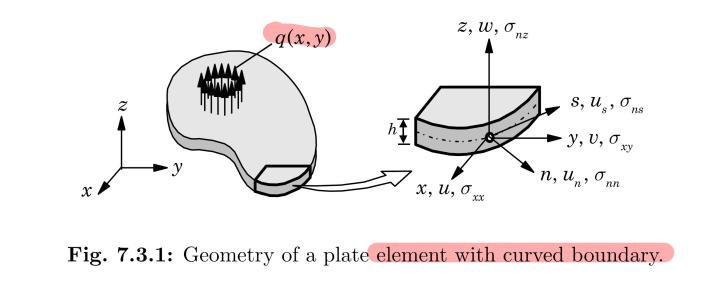
\includegraphics[width=0.8 \linewidth]{Figure/fig31} 		
			\end{figure}
		\end{itemize}
	\end{frame}


	\begin{frame}
		\begin{itemize}
			\item The principle of virtual work states that $0 = \delta W^e = \delta W_I^e + \delta W_E^e$
			\item As noted earlier, the transverse shears $\gamma_{xz},\gamma_{yz},\varepsilon_{zz}$ are zero. Therefore the transverse stresses ($\sigma_{xz},\sigma_{yz},\sigma_{zz}$ ) do not eneter the formulatin because the strains due to these are zero. Even though they are not accounted, in reality they exist to maintain equilibirum, these components can also be specified at the boudary. So they have to be accounted in the equilibirum equations. 
			\item The internal virtual strain is then given as 
			\begin{equation}
				\begin{aligned}
					\delta W_I^e = \int_A \int_{-\frac{h}{2}}^{\frac{h}{2}} 
					\left(
					\sigma_{xx} \delta \varepsilon_{xx} + \sigma_{yy} \delta \varepsilon_{yy} + 2\sigma_{xy} \delta \varepsilon_{xy}
					\right) dz~dx~dy\\
					= \int_A \left(N_{xx}\delta \varepsilon_{xx}^0 + M_{xx}\delta\varepsilon_{xx}^1 + N_{yy}\delta\varepsilon_{yy}^0 + M_{yy}\delta\varepsilon_{yy}^1 
					 + N_{xy}\delta\gamma_{xy}^0 + M_{xy}\delta\gamma_{xy}^1 \right) dx~dy
				\end{aligned}
			\end{equation}
			where N and M are the axial and the moment internal forces per unit length. 
		\end{itemize}
	\end{frame}


	\begin{frame}{Plate: Internal forces}
		\begin{figure}
			\centering
			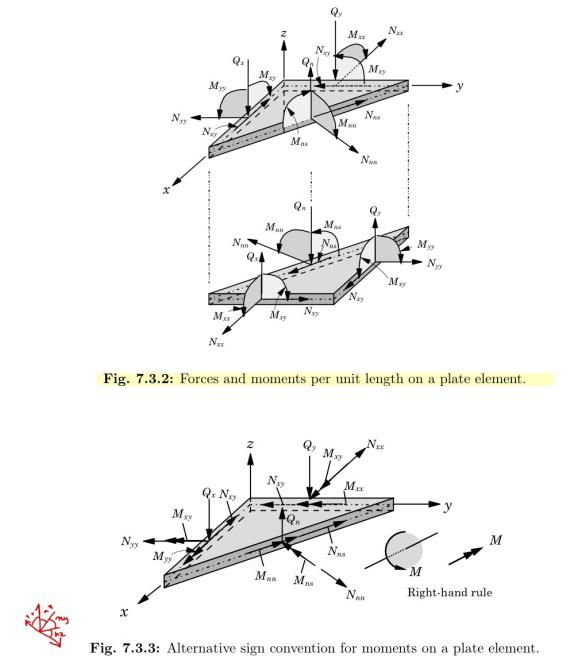
\includegraphics[width=0.6 \linewidth]{Figure/fig32} 		
		\end{figure}
	\end{frame}


	\begin{frame}
		\begin{itemize}
			\item The virtual work by the distributed transverse load q(x,y), reaction force of an elastic foundation, in plane normal stress $\sigma_{nn}$, in plane tangential stress $\sigma_{ns}$, transverse shear stress $\sigma_{nz}$ is 
			\begin{equation}
			\begin{aligned}
				\delta W_E^e = - (\int_A q(x,y) \delta w(x,y,\frac{h}{2}) dx~dy + 
				\int_A F_s(x,y) \delta w(x,y,-\frac{h}{2}) dx~dy
				\\	+ \int_S \int_{-\frac{h}{2}}^{\frac{h}{2}} \left[ \sigma_{nn} \left(\delta u_n - z \frac{\delta w}{n} \right) + \sigma_{ns} \left(\delta u_s - z \frac{\delta w}{s}\right) 
				+ \sigma_{nz}\delta w\right] dz~ds ) \\ 
				= - \left[ \int_S \left(N_{nn}\delta u_n - M_{nn}\frac{\partial \delta w}{\partial n}
							+ N_{ns}\delta u_s 
				            - M_{ns}\frac{\partial \delta w}{\partial s} + Q_n \delta w \right)ds
				            + \int_A (q-kw)\delta w dx~dy
				 \right] 
			\end{aligned}
			\end{equation}
			\item where Fs = -kw ( Foundation force), the negative sign it is the force applied upwards, but you can think of it like the potential increases as the w increases.
			\item The last term in the work term is the virtual work of the transverse and normal forces on a boundary that is inclined. Where N = $\int_{-\frac{h}{2}}^{\frac{h}{2}}\sigma$ ,  M = $\int_{-\frac{h}{2}}^{\frac{h}{2}}z\sigma$, $Q_n = \int_{-\frac{h}{2}}^{\frac{h}{2}}\sigma_{nz}$ 
		\end{itemize}
	\end{frame}


	\begin{frame}
	\begin{itemize}
		\item We now relate the stresses in the direction in the boundary to the internal stresses given in cartesion using stress tensor coordinate transformation
			\begin{equation}
			   \mat{\sigma_{nn}; \sigma_{ns}} = \mat{n_x^2,n_y^2,2n_xn_y ; -n_xn_y,n_xn_y,n_x^2 - n_y^2} \mat{\sigma_{xx};\sigma_{yy};\sigma_{xy}}
			\end{equation}
	\end{itemize}
	\end{frame}


	\begin{frame}{Weak forms}
		\begin{itemize}
			\item Keeping the weak forms in the full virtual work statement we get
			\begin{equation}
			\tiny
				\begin{aligned}
					0 =  \int_A \left(N_{xx}\delta \varepsilon_{xx}^0 + M_{xx}\delta\varepsilon_{xx}^1 + N_{yy}\delta\varepsilon_{yy}^0 + M_{yy}\delta\varepsilon_{yy}^1 
					+ N_{xy}\delta\gamma_{xy}^0 + M_{xy}\delta\gamma_{xy}^1 \right) dx~dy \\ - \left[ \int_S \left(N_{nn}\delta u_n - M_{nn}\frac{\partial \delta w}{\partial n}
					+ N_{ns}\delta u_s 
					- M_{ns}\frac{\partial \delta w}{\partial s} + Q_n \delta w \right)ds
					+ \int_A (q-kw)\delta w dx~dy
					\right]  \\ 
					 =  \int_A \left(N_{xx}\delta \varepsilon_{xx}^0 + M_{xx}\delta\varepsilon_{xx}^1 + N_{yy}\delta\varepsilon_{yy}^0 + M_{yy}\delta\varepsilon_{yy}^1 
					 + N_{xy}\delta\gamma_{xy}^0 + M_{xy}\delta\gamma_{xy}^1 \right) dx~dy \\ - \left[ \int_S \left(N_{nn}\delta u_n - M_{nn}\frac{\partial \delta w}{\partial n}
					 + N_{ns}\delta u_s 
					 - M_{ns}\frac{\partial \delta w}{\partial s} + Q_n \delta w \right)ds
					 + \int_A (q-kw)\delta w dx~dy
					 \right]  
				\end{aligned}
			\footnote{\tiny In the last three statements, It seems the equation has been kept according to the variation but how do you account for $ \delta u_n \quad \delta u_s$ as they will have components in both. Maybe the euler equations will make sense}
			\end{equation}
			
			\begin{figure}
				\centering
				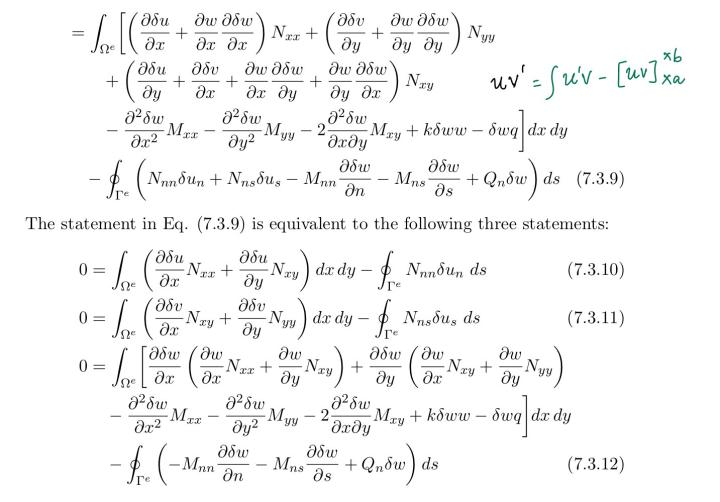
\includegraphics[width=0.6 \linewidth]{Figure/fig33} 		
			\end{figure}
	
		\end{itemize}
	\end{frame}


	\begin{frame}{Equilibrium equations}
		\begin{itemize}
			\item Keeping the virtual parameters in the same order to get the euler equations we get
			\begin{equation}
			\tiny
			\begin{aligned}
				0 = \int_A \left[ -\left(N_{xx,x} + N_{xy,y}\right)\delta u - \left( N_{xy,x} + N_{yy,y}\right)\delta v
		  			- \left(M_{xx,xx} + 2M_{xy,xy} + M_{yy,yy} + \mathcal{N} - kw + q\right) \delta w
							\right] dx~dy \\
				+ \int_S  (\left(N_{xx}n_x + N_{xy}n_y \right)\delta u  
			  + \left(N_{xy}n_x + N_{yy}n_y \right)\delta v
			  + \left( M_{xx,x}n_x + M_{xy,y}n_x + M_{yy,y}n_y + M_{xy,x}n_y + \mathcal{P} \right) \delta w \\
			  - \left(M_{xx}n_x + M_{xy}n_x \right)\frac{\partial \delta w}{\partial x} 
			  -\left(M_{xy}n_x + M_{yy}n_y \right)\frac{\partial \delta w}{\partial y} )ds  
			  -\int_S \left(N_{nn} \delta u_n + N_{ns}\delta u_s - M_{nn}\frac{\partial \delta w}{\partial n} - M_{ns}\frac{\partial \delta w}{\partial s} + Q_n \delta w \right)ds
			\end{aligned}
			\end{equation}
			\item Where 
				\begin{equation}
				\tiny
					\begin{aligned}
					\mathcal{N} = \frac{\partial }{\partial x} \left(N_{xx}\frac{\partial w}{\partial dx}   + N_{xy}\frac{\partial w}{\partial dy}\right)
					 + \frac{\partial }{\partial y} \left(N_{xy}\frac{\partial w}{\partial x} 
					+ N_{yy}\frac{\partial w}{\partial y}\right) \\
					\mathcal{P} = \left(N_{xx}\frac{\partial w}{\partial x}   + N_{xy}\frac{\partial w}{\partial y}\right) n_x
					+ \frac{\partial }{\partial y} \left(N_{xy}\frac{\partial w}{\partial x} 
					+ N_{yy}\frac{\partial w}{\partial y}\right) n_y 
					\end{aligned}
				\end{equation}
		\end{itemize}
	\end{frame}


	\begin{frame}
		\begin{figure}
			\centering
			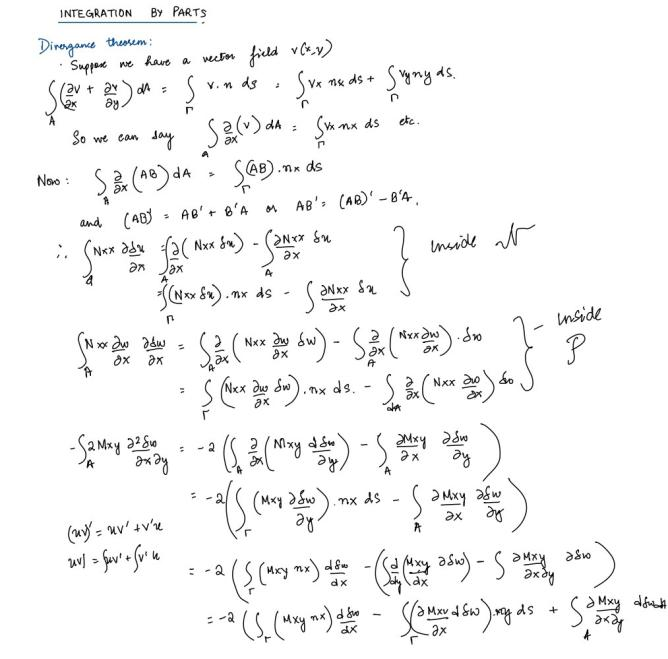
\includegraphics[width=0.7 \linewidth]{Figure/fig34} 		
		\end{figure}
	\end{frame}


	\begin{frame}{Euler-lagrange equilibrium equations}
		\begin{itemize}
			\item Keeping the coefficients of the variations (seting $\delta u, \delta v, \delta w = 0$)we get the equilibirum equations given as
			\begin{equation}
			\begin{aligned}
				\delta u : \frac{\partial N_{xx}}{\partial x} + \frac{\partial N_{xy}}{\partial y} = 0\\
				\delta v : \frac{\partial N_{xy}}{\partial x} + \frac{\partial N_{yy}}{\partial y} = 0\\
				\delta w : \frac{\partial^2 M_{xx}}{\partial x^2} + 2\frac{\partial^2 M_{xy}}{\partial x \partial y} + \frac{\partial^2 M_{yy}}{\partial y^2} + \mathcal{N} - kw + q = 0
			\end{aligned}
			\end{equation}
		\end{itemize}
	\end{frame}


	\begin{frame}{Boudnary conditions}
		\begin{itemize}
			\item To cast the B.C. on an edge whose normal is $\ve{n}$, we express the generalised displacements ($u,v,w,\frac{\partial w}{\partial x}, \frac{\partial w}{\partial y}$) in x,y,z system in the corresponding displacements in normal, tangential and transverse directions. We get
			\begin{equation}
			\begin{aligned}
				u = u_nn_x - u_sn_y \qquad v = u_nn_y + u_sn_x \\ 
				\frac{\partial w}{\partial x} = \frac{\partial w}{\partial n} n_x 
				- \frac{\partial w}{\partial s}n_y \qquad 
				\frac{\partial w}{\partial y} = \frac{\partial w}{\partial n}n_y
				+ \frac{\partial w}{\partial s}n_x
			\end{aligned}
			\end{equation}
			\begin{figure}
				\centering
				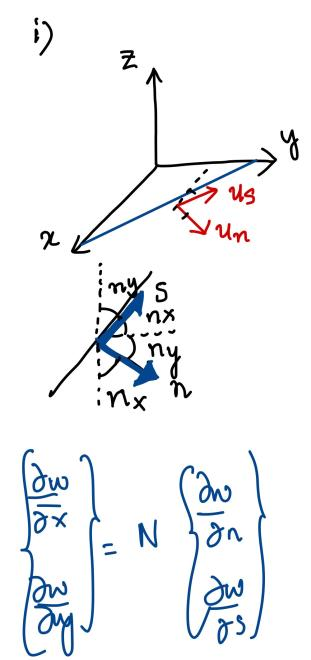
\includegraphics[width=0.2  \linewidth]{Figure/fig35} 		
			\end{figure}
		Now the derivative of $w$ is a vector which can undergo basis transformation
 		\end{itemize}
	\end{frame}


	\begin{frame}{Boundary conditions}
		\begin{itemize}
			\item The boundary conditions can be written in the normal, tangenetial coords 
			\begin{equation}
			\tiny
			\begin{aligned}
			\int_S [ 
			\left(N_{xx}n_x + N_{xy}n_y\right)\left(\delta u_nn_x - \delta u_sn_y\right) +
			\left(N_{xy}n_x + N_{yy}n_y\right)\left(\delta u_nn_y + \delta u_sn_x\right) \\ +
			\left( M_{xx,x}n_x + M_{xy,y}n_x + M_{yy,y}n_y + M_{xy,x}n_y + \mathcal{P} \right) \delta w \\ - 
			\left(M_{xx}n_x + M_{xy}n_y \right)\left(\frac{\partial w}{\partial n} n_x 
			- \frac{\partial w}{\partial s}n_y \right) - 
			\left(M_{xy}n_x + M_{yy}n_y \right)\left(\frac{\partial w}{\partial n} n_y 
			+ \frac{\partial w}{\partial s}n_x \right)]ds\\
			 - \int_S \left(N_{nn} \delta u_n + N_{ns}\delta u_s - M_{nn}\frac{\partial \delta w}{\partial n} - M_{ns}\frac{\partial \delta w}{\partial s} + Q_n \delta w \right)ds
			\end{aligned} 
			\end{equation}
			\item $\delta u$ in natural does not change the direction cosines because here they are constant dependant on the geometry we are at and not the variation.
		\end{itemize}
	\end{frame}


	\begin{frame}{Boundary conditions}
		\begin{figure}
			\centering
			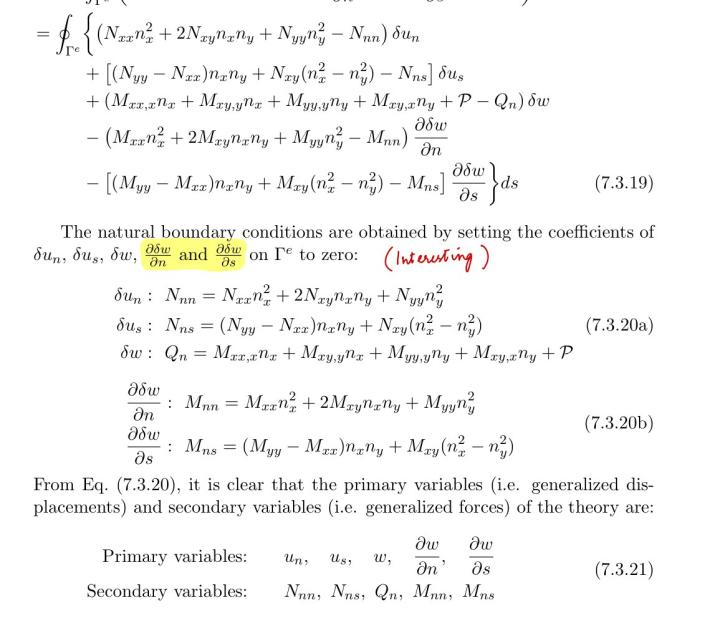
\includegraphics[width=0.7\linewidth]{Figure/fig36} 		
		\end{figure}
		\begin{itemize}
			\tiny
			\item I find this interesting to keep the varitaion with derivatives equal to zero.
			\item We see that from the equilibrium equations, if we keep them in displacements we woul get a DE having second order spatial derivatives of u, v and fourth order of w. Therefore we need eight boundary conditions (4 primary and 4 natural). But we have eight
		\end{itemize}
	\end{frame}


	\begin{frame}{Kirchoff free-edge condition}
		\begin{itemize}
			\item To remove this problem, one can integrate the tangential derivative term by parts
			\begin{equation}
				-\int_S M_{ns}\frac{\partial \delta w}{\partial s} ds = \int_S \frac{\partial M_{ns}}{\partial s}\delta w ds - [M_{ns}\delta w]_{\Gamma}
			\end{equation}
			\item The second term [$M_{ns}\delta w$] is zero when the end points of two curves meet or when $M_{ns} = 0$. If $M_{ns}$ is not specified at the corners, then concentrated forces $F = -2M_{ns}$ are produced at the corners. 2 appears from the two sides of the corner. 
			\item The remaining boundary term is added to the shear force $Q_n$ (Also having a coefficien of $\delta w$ in integral  S)to get
			\begin{equation}
				V_n = Q_n + \frac{\partial M_{ns}}{\partial s}
			\end{equation}
			This specification of theshare force is known a sthe Kirchoff free edge condition. The final boundary conditions are 
			\begin{equation}
			\begin{aligned}
			\text{Genearlised dispalcements} : u_n, u_s,w,\frac{\partial w}{\partial n} \\
			\text{Generalised forces} : N_{nn}, N_{ns}, V_n, M_{nn}
			\end{aligned}
			\end{equation}
			\footnote{So you known either one he displacement of the forces. On a side parallel to x asix (s = x and n =y). $u_n =v, u_s = u, w, \frac{\partial w}{\partial n} = \frac{\partial w}{\partial y}, N_{nn}=N_{yy},N_{ns}=N_{yx}, V_n =V_y,M_{nn}=M_{yy}$}
		\end{itemize}
	\end{frame}


	\begin{frame}{Typical edge conditions}
		We discuss for some common boundary with edges parallel to x and y coordinates
		\begin{itemize}
			\item \textbf{Free edge with normal $\ve{n}$} : We don't know the disp but we know the force/moment
			\begin{equation}
				\begin{aligned}
				u_n \neq 0, \quad u_s \neq 0, \quad w \neq 0, \quad \frac{\partial w}{\partial n} \neq 0 \\
				N_{nn} = \hat{N_{nn}}, \quad N_{ns} = \hat{N_{ns}}, V_n =  Q_n + \frac{\partial M_{ns}}{\partial s} = \hat{V_n}, M_{nn} = \hat{M_{nn}}
				\end{aligned}
			\end{equation}
			\item \textbf{Fixed with normal $\ve{n}$} : Fixed edge with primary values known. But we dont know the reaction forces and moments. Given as \\
			$u_n =0, \quad u_s =0,\quad w = 0,\quad \frac{\partial w}{\partial n} = 0 $. 
			\item \textbf{Simply suppored} : This is not unize especially when both inplane and bending are coupled. Here showing two types
			\begin{enumerate}
				\item SS1: $u_s = 0, \quad w =0 \quad, N_{nn}=\hat{N_{nn}}, \quad M_{nn} = \hat{M_{nn}}$
				\item SS2: $u_n = 0, \quad w =0 \quad, N_{ns}=\hat{N_{ns}}, \quad M_{nn} = \hat{M_{nn}}$
			\end{enumerate}
			
		\end{itemize}
	\end{frame}


	\begin{frame}{Stress resultant-Deflection relations}
		\begin{itemize}
			\item To express the foces and moments (N,M) per unit length in terms of the generalized displacements we need to bring the correct stress-strain relations. In the classical plate theory all the transverse strain components ($\varepsilon_{xx,xz,yz}$) are zero.
			\item  Since $\varepsilon_{zz} = 0$, the transverse normal stress $\sigma_{zz}$ even though not zero, does not appear in the virtual work statement and equation of motion. Therefore it is like we are neglecting the transverse normal stress. So we have a case of both plane strain and plane sterss.
			\item From practical consideration however a thin/moderatel thick plate is in plane stress because the thickness is smaller.
			
		\end{itemize}
	\end{frame}


	\begin{frame}{Constitutive relations}
		\begin{itemize}
			\item Orthotropic material with principal axes ($x_1,y_1,z_1$) coincident with the plate coordinates (x,y,z), we get
			\begin{equation}
			\mat{\sigma_{xx};\sigma_{yy};\sigma_{xy}} = \mat{Q_{11},Q_{12},0;Q_{12},Q_{22},0;0,0,Q_{66}}
			\mat{\varepsilon_{xx} - \alpha_1\Delta T;\varepsilon_{yy} - \alpha_2\Delta T;\gamma_{xy}}
			\end{equation}
			where 
			\begin{equation}
			\begin{aligned}
			Q_{11} =  \frac{E_1}{1-\nu_{12}\nu_{21}} \qquad Q_{12} =  \frac{\nu_{12} E_2}{1-\nu_{12}\nu_{21}} = \frac{\nu_{21} E_1}{1-\nu_{12}\nu_{21}} \\
			Q_{22} = \frac{E_2}{1-\nu_{12}\nu_{21}} \qquad Q_{66} = G_{12}
			\end{aligned}
			\end{equation}
			\item The temperature increment is froma reference state.
		\end{itemize}
	\end{frame}


	\begin{frame}{Force-displacement}
		\begin{itemize}
			\item Now we can relate the forces, moments per unit length to the strains. Integrating the stresses over the cross section gives the required axial force and moments (With the lever arm z). 
			\item For plates that are laminated with multiple orthotropoic layers, whose material axes are \textbf{arbitrarily} oriented with respect to the plate eaxes, the constitutive relations couple the inplane and out of plane displacements even for linear prolbems
			\item For a single orthortropic layer, the constitutive relations are simplified as :
		\end{itemize}
		\begin{figure}
			\centering
			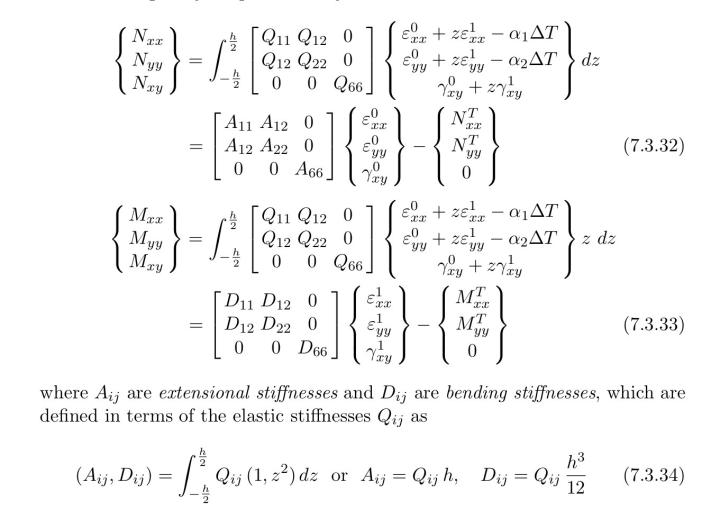
\includegraphics[width=0.55\linewidth]{Figure/fig37}  	
			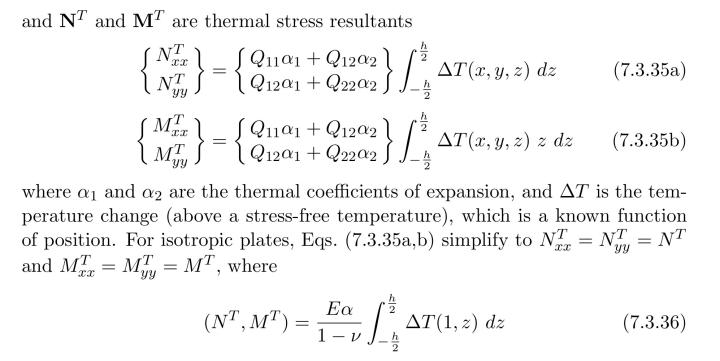
\includegraphics[width=0.4\linewidth]{Figure/fig38}	
		\end{figure}
	\end{frame}


	\begin{frame}{FEM}
		\begin{figure}
			\centering
			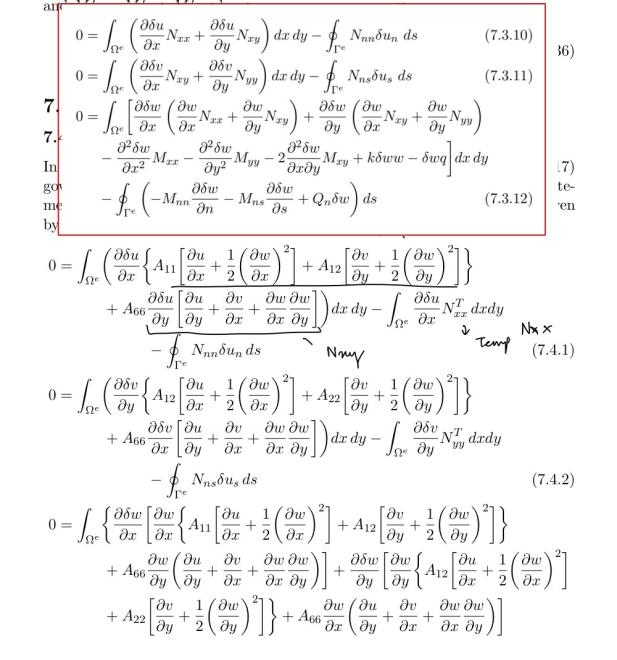
\includegraphics[width=0.6\linewidth]{Figure/fig39}  		
		\end{figure}
	\end{frame}


	\begin{frame}
		\begin{itemize}
			\item We know that $u_n,~u_s,~w,~\frac{\partial w}{\partial n}$ are used as primary variables ( or gerneralised displacements)
			\item $\hat{N_{nn}},\hat{N_{ns}},\hat{V_{n}},\hat{M_{nn}}$ as secondary degrees of greedom (generalised forces)
			\item The finite elements based on the transverse deflection $w$ and its derivative acroos element boundary (C1 conitunity). In completeness, it should be a full quadratic.
			\item $u_n$ and $u_s$ need only be C0. We shall use $u,v,w,\frac{\partial w}{\partial x}, \frac{\partial w}{\partial y}$ as the generalised displacements. We assume as
			\begin{equation}
			u(x,y) =N_i^1u_i \qquad v(x,y)=N_i^1u_i \qquad w(x,y) = N_i^2u_i
			\end{equation}
			\item In case of a rectangular element wecan take two sets of dof at each node : $u,,v,w,w_{,x},w_{,y}$ and $u,,v,w,w_{,x},w_{,y}, w_{,xy}$ called non conforming and conforming element. 
			\item  In substituting we get
			\begin{equation}
				\ve{\mat{K_{11},K_{11},K_{11};K_{21},K_{22},K_{23};K_{31},K_{32},K_{33}} \mat{u;v;\Delta} = \mat{F_1;F_2;F_3} + \mat{F_{1T};F_{ 2T};F_{3T}} }
			\end{equation}
			
		\end{itemize}
	\end{frame}


	\begin{frame}
		\begin{figure}
			\centering
			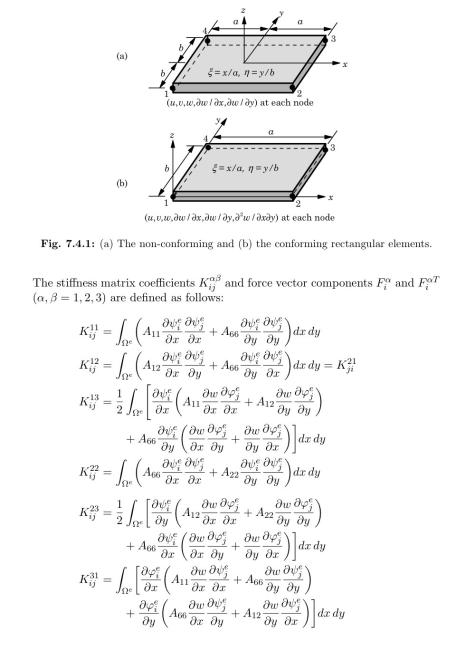
\includegraphics[width=0.4\linewidth]{Figure/fig40}  		
			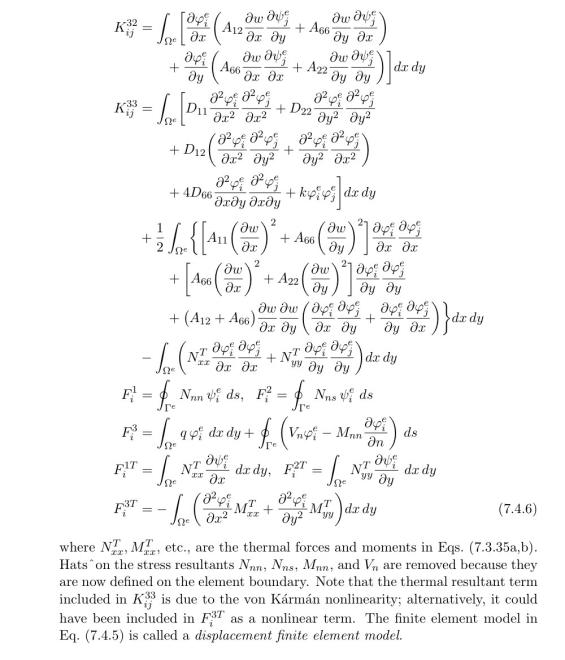
\includegraphics[width=0.4\linewidth]{Figure/fig41}
		\end{figure}
	\end{frame}


	\begin{frame}{Tangent stiffness coefficients}
		\begin{itemize}
			\item Check Tangent in Reddy 328
		\end{itemize}
	\end{frame}


	\begin{frame}{Conforming and non conforming plate elements}
		\begin{itemize}
			\item A non conforming element also has nodal variable of $w_{,x},w_{,y}$
			\item Using the parametric form we see that 
			\begin{equation}
				\begin{aligned}
				u = u_h =  u_i N^1_i(\xi,\eta) \qquad v = v_h =  v_iN^1_i(\xi,\eta) \\
				w_h = \Delta N^2_i(\xi,\eta) ~~\text{Cubic to associate with dof}~ w,w_{,x},w_{,y}\\			
				\end{aligned}
			\end{equation}
			\item The variation of the normal slope $w_{,n}$ is cubic while there are only two values of it available on the edge ()??????????.
			\item Therefore, cubic polynomials for the normal derivatives of $w$ are not the same on an edge common to two elements, hence non-conforming. I guess corner one is not the same 
			\item Conforming elemen has $w$ approximated by 16 term complete polyunomial with dof $w, w_{,x},w_{,y},w_{,xy}$
			\item Here the normal slope continuity between elements is satisfied.
			\end{itemize}
	\end{frame}


	\begin{frame}{Derivatives}
		\begin{itemize}
			\item Here we use bilinear interpolation of $u,v$ and hermite of $w$
			\item The geomettry is also represented using bilinear interpolating functions
			\begin{equation}
				x = N_i(\xi,\eta)x_i \qquad y = N_i(\xi,\eta) y_i
			\end{equation}
			\item The derivatives of the inerpolating funcction with respect to global is given by
			\begin{equation}
				\mat{\frac{\partial N_i}{\partial x}; \frac{\partial N_i}{\partial y} = J^{-1} 
					\mat{\frac{\partial N_i}{\partial \xi}; \frac{\partial N_i}{\partial \eta}}}
			\end{equation}
			\item For the second order derivatives, we can use again chain rule
			\begin{equation}
			\begin{aligned}
				\frac{\partial N_i}{\partial \xi} = \frac{\partial N_i}{\partial x}\frac{\partial  x}{\partial \xi} + \frac{\partial N_i}{\partial y}\frac{\partial  y}{\partial \xi}
				\qquad
				\frac{\partial N_i}{\partial \eta} = \frac{\partial N_i}{\partial x}\frac{\partial  x}{\partial \eta} + \frac{\partial N_i}{\partial y}\frac{\partial  y}{\partial \eta} \\
				\frac{\partial^2 N_i}{\partial \xi^2} = \frac{\partial }{\partial \xi}\left(\frac{\partial N_i}{\partial x}\frac{\partial  x}{\partial \xi} + \frac{\partial N_i}{\partial y}\frac{\partial  y}{\partial \xi} \right)		\qquad
				\frac{\partial^2 N_i}{\partial \eta^2} = \frac{\partial }{\partial \eta}\left(\frac{\partial N_i}{\partial x}\frac{\partial  x}{\partial \eta} + \frac{\partial N_i}{\partial y}\frac{\partial  y}{\partial \eta} \right)		  
			\end{aligned}
			\end{equation}
		\end{itemize}
	\end{frame}


	\begin{frame}{Stresses}
		\begin{itemize}
			\item The stresses $\sigma_{xx},\sigma_{yy},\sigma_{xy}$ are computed using stress-strain relations and computed in global coordinates using 		
		\end{itemize}
		\begin{figure}
			\centering
			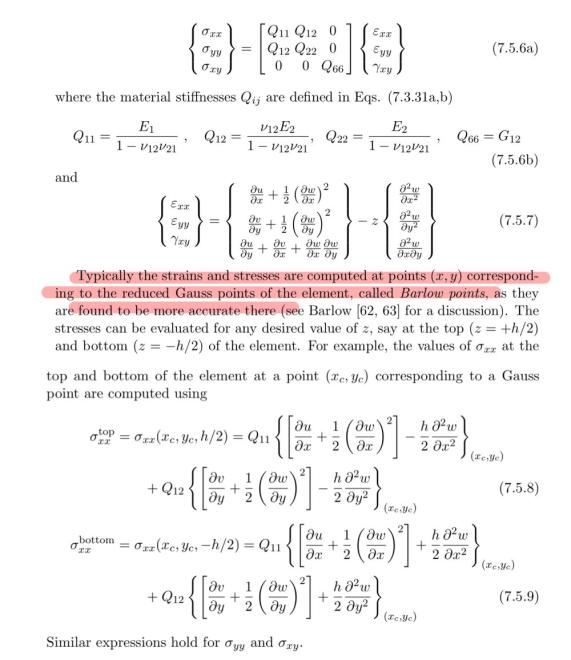
\includegraphics[width=0.5\linewidth]{Figure/fig42}  		
		\end{figure}
	\end{frame}

	
	\begin{frame}{First order shear deformation}
		\begin{itemize}
			\item Transverese normal and shear are not neglected. This formulation requires only C0 interpolation of all gerneralized displacements!
			\item Displacement field : Same assumptions of classical theroy but relaxing the normality condition
			\begin{equation}
			\begin{aligned}
				u_1(x,y,z) = u(x,y) + z\phi_x(x,y)\\
				u_2(x,y,z) = v(x,y) + z\phi_y(x,y)\\
				u_3(x,y,z) = w(x,y) 
			\end{aligned}
			\end{equation}
			\begin{figure}
				\centering
				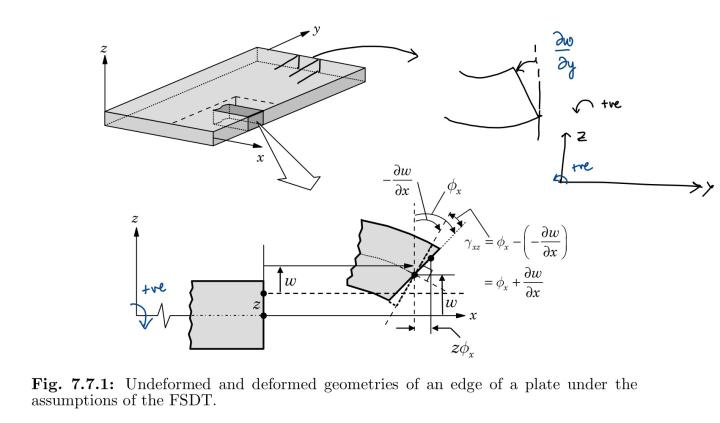
\includegraphics[width=0.55\linewidth]{Figure/fig44}  		
			\end{figure}
			\item Where ($u,v,w,\phi_x,\phi_y$) are unkown functions. $\phi_x,\phi_y$ denote the rotations of transverser normal line about y and x axes. These are called generalized displacements
		\end{itemize}
	\end{frame}


	\begin{frame}{Displacement: Continued}
		\begin{itemize}
			\item Notation that $\phi_x,\phi_y$ denoe rotation about a transverse normal about y
			\item We then get
			\begin{equation}
			\begin{aligned}
				\beta_x = -\phi_y \qquad \beta_y = \phi_x\\
				\phi_x = - \frac{\partial w}{\partial x} \qquad 				
				\phi_y = - \frac{\partial w}{\partial y} \quad \text{For thin plates of thickness ratio of order \~ O(50)}
			\end{aligned}
			\end{equation}
			\item However this equality is not achieved in the discrete fem model, resulting in shear locking as in Timoshenko beam, when the same lower order approx are used for transverse deflection $w$ and rotation $\phi$
			
		\end{itemize}
	\end{frame}


	\begin{frame}{von Karman strains}
		\begin{itemize}
			\item The von karman strains are:
			\begin{equation}
			\mat{\varepsilon_{xx};\varepsilon_{yy};\varepsilon_{yz};\varepsilon_{xz};\varepsilon_{xy}} =
			\mat{\varepsilon^0_{xx};\varepsilon^0_{yy};\varepsilon^0_{yz};\varepsilon^0_{xz};\varepsilon^0_{xy}} +
		z   \mat{\varepsilon^1_{xx};\varepsilon^1_{yy};0;0;\varepsilon^1_{xy}} =
			\mat{\frac{\partial u}{\partial x} + \frac{1}{2}(\frac{\partial w}{\partial x})^2 ; ; 
				 \frac{\partial v}{\partial y} + \frac{1}{2}(\frac{\partial w}{\partial y})^2 ; ;
			     \frac{\partial w}{\partial y} + \phi_y                                       ; ;
		     	 \frac{\partial w}{\partial x} + \phi_x                                       ; ;
	     	     \frac{\partial u}{\partial y} + \frac{\partial v}{\partial x} + \frac{\partial w}{\partial x} \frac{\partial w}{\partial y}} +
        z   \mat{\frac{\partial \phi_x}{\partial x}; ; \frac{\partial \phi_y}{\partial y}; ; 0 ; ; 0 ; ; \frac{\partial \phi_x}{\partial y} + \frac{\partial \phi_y}{\partial x}}
			\end{equation}
			\item Note that the strains ($\varepsilon_{xx,yy,xy}$) are linear through the plate thickness while the transverse strains ($\gamma_{xz},\gamma_{yz}$) are constant.
		\end{itemize}
	\end{frame}


	\begin{frame}{Weak form using virtual work}
		\begin{itemize}
			\item The weak form for $\delta W_I$ and $\delta W_E$ is :
			\begin{figure}
				\centering
				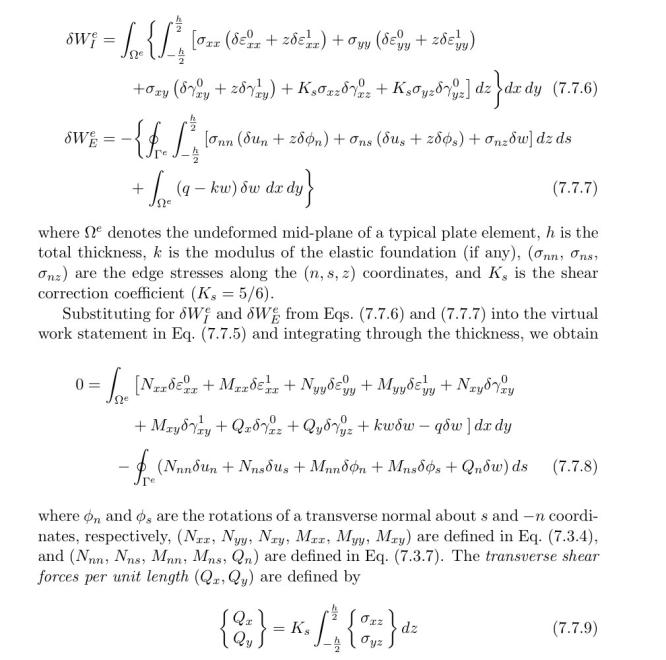
\includegraphics[width=0.7\linewidth]{Figure/fig45}  		
			\end{figure}
		\end{itemize}
	\end{frame}


	\begin{frame}{Governing equationbs}
		\begin{itemize}
			\item The virtual work equation contains five different statements associated with five virtual displacements ($\delta u, \delta v, \delta w, \delta \phi_x, \delta \phi_y$) forming the basis of the fem model
			\item The governing equations not required for fem, are shown as done previously by removing all the virtual displacments of differentiation. We then get:
		\end{itemize}
	\end{frame}


	\begin{frame}
		\begin{figure}
			\centering
			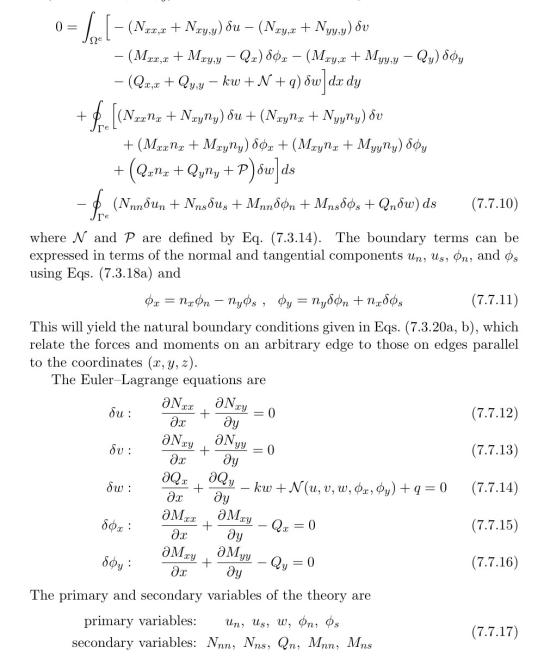
\includegraphics[width=0.65\linewidth]{Figure/fig46}  		
		\end{figure}
	\end{frame}


	\begin{frame}
		\begin{itemize}
			\item Since the transverse shear strains are constant, the shear stresses will also be constant. But the transverse shear stress is actually parabolic, whihc is taken care using a shape factor on the shear stiffness. 
			\begin{figure}
				\centering
				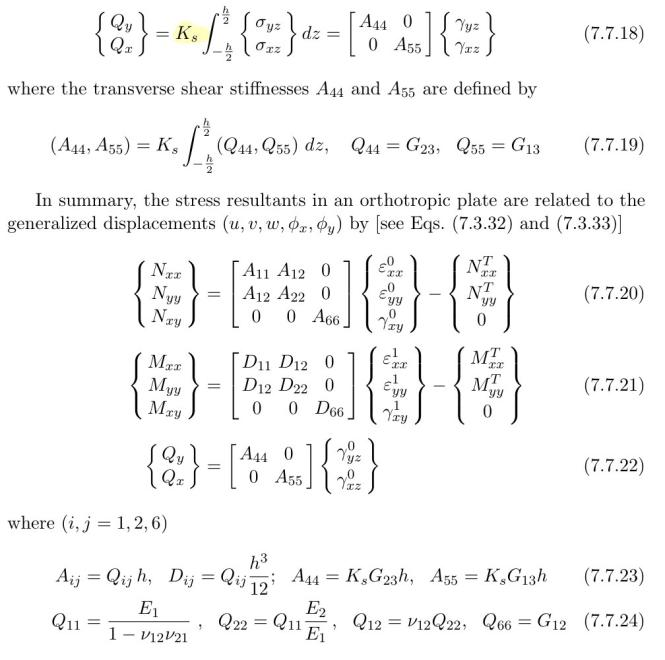
\includegraphics[width=0.65\linewidth]{Figure/fig47}  		
			\end{figure}
			\item As you can see that once you have the shear deformation, we change how G (shear modulus is)
		\end{itemize}
	\end{frame}


	\begin{frame}{FEM models of FSDT}
		\begin{itemize}
			\item FEM model
			\item  The rotationsa ($\phi$) are independant of $w$. So no derivatives appear and all the  generalized displafcements can be interpolated using Largrange interpolating functions.
			\item Tangent matrix : See Reddy
			
		\end{itemize}
	\end{frame}


	\begin{frame}{Shear and membrane locking and transient}
		\begin{itemize}
			\item The lienarised interpolation of the generalized displcamnets is used, making the element very stiff in the thin plate limit. This is called shear locking. A common technique is to use selective integration. Reduced integration is used to evalueate all the transeverse shear stiffnesses.			
			\item \textbf{Transient:}Check Reddy
	\end{itemize}
	\end{frame}

	\begin{frame}{Example 7.6.1}
		\begin{itemize}
			\item 
			
		\end{itemize}
	\end{frame}
\end{document}


